\chapter{Anforderungsanalyse}\label{anforderungsanalyse}
\section{Einleitung}
\subsection{Zweck}
Die Anforderungsanalyse dient als Basis für die folgenden Abschnitte:

\begin{itemize}
	\item \textbf{Architektur und Konzept:}  Die dokumentierten Anforderungen dienen als Grundlage für die Architektur des Systems und das Konzept. 
	\item \textbf{Implementation:} Die Implementation der Anwendung richtet sich nach den ermittelten Anforderungen. 
	\item \textbf{Verifikation:} Der implementierte Software-Prototyp wird anhand der in diesem Abschnitt ermittelten Anforderungen bewertet. 
\end{itemize}

\subsection{Systemumfang}
Der folgende Abschnitt beschreibt die wesentlichen Teile innerhalb des Systems und des Systemkontexts. 
 \begin{figure}[H]
  	\centering
    	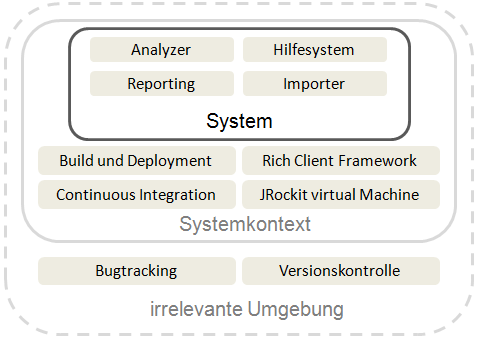
\includegraphics{images/systemumfang}
        	\caption{System und Systemkontext}
\end{figure}
\subsubsection{System}
Das System besteht aus den Teilen Datenmodell, Domäne, Log Parsing, Garbage Collection Analyse, Report, Charting, Hilfesystem\footnote{Dem Benutzer wird sowohl eine generelle wie auch eine kontextbezogene Hilfe angeboten.}, Benutzerführung.

\subsubsection{Systemkontext}
Zum Systemkontext gehören folgende nicht veränderbare Komponenten:
\begin{itemize}
	\item \textbf{Build und Deployment, Continuous Integration:} Der Build der Software für neue Updates oder Releases wird zentral auf einem Server durchgeführt. Der Source-Code wird aus der Versionskontrolle ausgecheckt, die binären Packete werden gebildet, es wird ein für den jeweiligen Update-Mechanismus notwendiges Packet erstellt und auf den Update-Server gestellt.

	\item \textbf{Update Mechanismus:} Die Software wird in der Version 1.0 released. Anschliessend können Updates (Minor-, Major-Versionen) direkt - ohne den manuellen Download der Software - durchgeführt werden.
	\item \textbf{JRockit Virtual Machine:} Die Schnittstelle zur JRockit Virtual Machine findet über deren Logdateien statt. Die genaurere Beschreibung befindet sich unter \titleref{jrockitgclog}.
\end{itemize}

\subsubsection{Irrelevante Umgebung}
\begin{itemize}
	\item \textbf{Bugtracking:} Sobald die Software stabil läuft und an Tester herausgegeben wird, wird für die Verwaltung der Fehler (Bugs) ein Bugtracker verwendet.
	\item \textbf{Versionskontrolle:} Der Source-Code der Applikation wird in einer Source-Code-Verwaltung abgelegt. Diese dient als Backup und zur Versionierung der einzelnen Artefakte. Die beiden Werkzeuge (Bugtracker, Versionskontrolle) arbeiten normalerweise eng zusammen, so dass Bug Fixes mit der eingecheckten Version in Verbindung bleiben.
\end{itemize}


\subsection{Stakeholder}
Für die Anforderungsanalyse sind nur die mit Asteriks gekennzeichneten Stakeholder-Rollen relevant. Die anderen Rollen können erst dann berücksichtigt werden, wenn die Software eine weitere Verbreitung wahrnehmen kann. Verschiedene Rollen können auch von einer Person wahrgenommen werden. 
\begin{figure}[H]
  	\centering
    	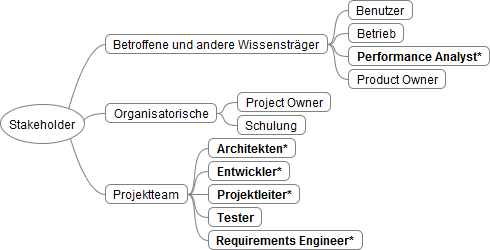
\includegraphics[width=13cm]{images/stakeholder_analyse}
        	\caption{Übersicht der Stakeholder}
\end{figure}

\subsection{Glossar}
Das Glossar befindet sich auf Seite \pageref{glossar}. 
\subsection{Referenzen}
Die Referenzen innerhalb des Abschnitts \titleref{anforderungsanalyse} befinden sich im Abschnitt Literaturverzeichnis.
\subsection{Übersicht}
Die Anforderungsanalyse ist folgendermassen aufgebaut: Beginnen tut sie mit der Allgemeinen Übersicht. Hier sind Architektur, Nutzer- und Zielgruppen, Randbedingungen und Annahmen dokumentiert. Danach sind die Use Cases der Software beschrieben. Aus diesen leiten sich dann die funktionalen Anforderungen und schliesslich die Qualitätsanforderungen ab.
\section{Allgemeine Übersicht}\label{allgemeine_uebersicht}
\subsection{Architekturbeschreibung}
Die Software wird als Plugin programmiert. Der Entwickler kann sich die Software als Erweiterung in seiner Entwicklungsumgebung installieren. Sobald die Software installiert ist, wird für die Arbeit keine Verbindung ins Internet mehr benötigt. Die Applikation ist auf allen gängigen Betriebssystemen (Linux, Mac OSX, Windows) lauffähig.

\subsection{Nutzer und Zielgruppen}
\subsubsection{Performance Engineers}
Normalerweise Software Entwickler die viel Erfahrung, Wissen, Fähigkeiten haben und über die entsprechenden Werkzeuge verfügen, um die Ursachen für Performance-Probleme zu finden. Dabei handelt es sich nicht nur um Wissen im Bereich der Softwareentwicklung, sondern auch im Bereich des Servers und des Betriebssystems (Speichermanagement, I/O, etc.). Durch ihr breites Wissen sind sie mit der Unterstützung von Charts, Statistiken und Reports schnell in der Lage, Ursache von Performanceproblemen zu finden.

\subsubsection{Java Entwickler}
Im Gegensatz zu Performance Engineers beschäftigen sich Java Entwickler vorallem mit der Entwicklung von Anwendungen und verfügen nicht direkt über Knowhow im Bereich der Performanceanalyse. Als gut ausgebildete Ingenieure sind sie aber mit Hilfe von Werkzeugen und Dokumentation in der Lage, Performance Problemen innert nützlicher First auf den Grund zu gehen.

\subsection{Randbedingungen}\label{randbedingungen}
Das Format der Logdatei der JRockit Virtual Machine hat sich im Bereich des Memory Managements von der Version R27 auf die Version R28 geändert. Die Kompatibilität mit Versionen älter als R28 wird vorerst nicht gegeben sein.
\subsection{Annahmen}


\section{Use Cases}\label{use_cases}
\subsection{Systemfunktionalität}\label{systemfunktionalitaet}
 \begin{figure}[H]
  	\centering
    	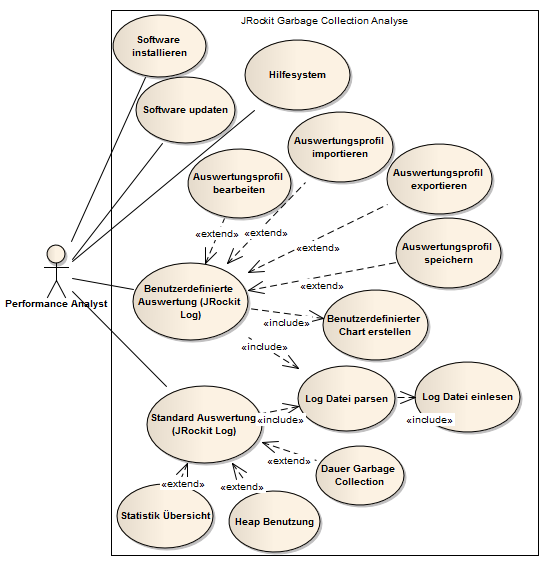
\includegraphics[width=14cm]{images/anforderungen_use-case}
        	\caption{Systemfunktionalität als Use-Case-Diagramm}
\end{figure}
Die ersten beiden Teile dieses Abschnitts definieren die Use Cases des Systems. Als Basis dient die Schablone zur Use-Case-Spezifikation in \cite[S. 78-79]{pohl2010basiswissen}.
\section{Use Cases}\label{use_cases}
Dieser Abschnitt zeigt die Use Cases für die Analysesoftware. Daraus werden dann im nächsten Abschnitt die Anforderungen respektive die finale Anforderungsliste abgeleitet. Als Einstieg dient das UML Use Case Diagramm, in welchem die Systemgrenzen, der Anwender (Performance Analyst) und die verschiedenen Use Cases dargestellt sind. Die einzelnen Use Cases sind dann nach der in \cite[S. 78-79]{pohl2010basiswissen} beschriebenen Schablone definiert.
\subsection{Übersicht}\label{systemfunktionalitaet}
 \begin{figure}[H]
  	\centering
    	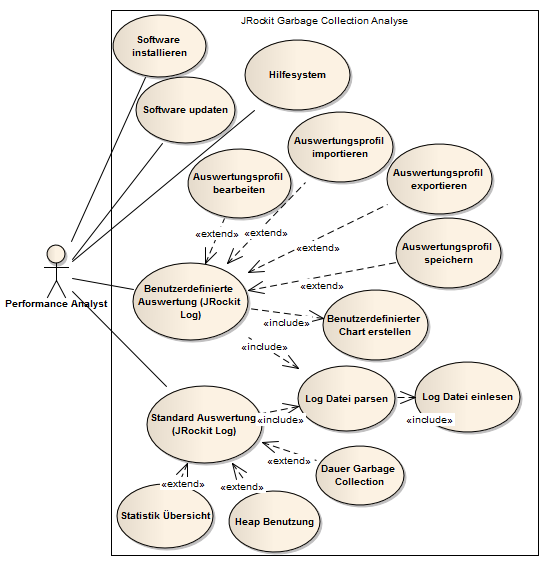
\includegraphics[width=14cm]{images/anforderungen_use-case}
        	\caption{Systemfunktionalität als Use-Case-Diagramm}
\end{figure}
\subsection{Beschreibung}
Die definierten Use Cases leiten sich aus einer Anforderung ab, welche über die Nummer referenziert ist.
\begin{longtable}{|p{4cm}|p{10.5cm}|}
  \hline
   \textbf{Abschnitt} & \textbf{Inhalt / Erläuterung} \\\hline
   Bezeichner & UC-01\\\hline
   Name & Software installieren\\\hline
   Autoren & Raffael Schmid\\\hline
   Priorität & Wichtigkeit für Systemerfolg: gross\newline Technologisches Risiko: mittel\\\hline
   Kritikalität & gross\\\hline
   Verantwortlicher & Raffael Schmid\\\hline
   Kurzbeschreibung & Der Benutzer kann die Software in seiner Entwicklungsumgebung installieren.\\\hline
   Akteure & Anwender, Entwicklungsumgebung\\\hline
   Auslösendes Ereignis & Anwender möchte eine Garbage Collection Logdatei analysieren.\\\hline
   Vorbedingung & Richtige Entwicklungsumgebung ist bereits ohne Analysesoftware installiert.\\\hline
   Nachbedingung & Es sind keine Fehler aufgetreten.\\\hline
   Ergebnis & Entwicklungsumgebung ist bereit für Garbage Collection Auswertungen.\\\hline
   Hauptszenario & 
         \begin{enumerate}
		\item Anwender Startet Entwicklungsumgebung
		\item Anwender gibt Update-Seite an
		\item Anwender selektiert zu installierendes Softwarepaket
		\item Softwarepaket wird installiert	
 	\end{enumerate}
	\\\hline
   Alternativszenarien & -\\\hline
   Ausnahmeszenarien & -\\\hline
   Qualitäten & Usability\\\hline
\caption{Use-Case: Software installieren}
\end{longtable}

\begin{longtable}{|p{4cm}|p{10.5cm}|}
\hline
   \textbf{Abschnitt} & \textbf{Inhalt / Erläuterung} \\\hline
   Bezeichner & UC-02\\\hline
   Name & Software updaten\\\hline
   Autoren & Raffael Schmid\\\hline
   Priorität & Wichtigkeit für Systemerfolg: gross\newline Technologisches Risiko: mittel\\\hline
   Kritikalität & Mittel\\\hline
   Verantwortlicher & Raffael Schmid\\\hline
   Kurzbeschreibung & Der Benutzer kann die Software updaten.\\\hline
   Akteure & Anwender, Update-Server\\\hline   
   Auslösendes Ereignis & Anwender hat die Software bereits zu einem früheren Zeitpunkt installiert. Sofern ein neues Update vorhanden ist, möchte er dieses installieren.\\\hline
   Vorbedingung & Richtige Entwicklungsumgebung und Software wurden bereits in einer früheren Version installiert.\\\hline
   Nachbedingung & Es sind keine Fehler aufgetreten.\\\hline
   Ergebnis & Entwicklungsumgebung und Analysesoftware sind auf dem neusten Stand für Garbage Collection Auswertungen.\\\hline
   Hauptszenario & 
	\begin{enumerate}
		\item Anwender Startet Entwicklungsumgebung
		\item Anwender sucht und findet Updates für die Analysesoftware
		\item Anwender selektiert eines oder mehrere dieser Softwarepakete
		\item Software wird aktualisiert
	\end{enumerate}
	\\\hline
   Alternativszenarien & -\\\hline
   Ausnahmeszenarien & -\\\hline
   Qualitäten & Usability\\\hline
\caption{Use-Case: Software updaten}
\end{longtable}

\begin{longtable}{|p{4cm}|p{10.5cm}|}
\hline
   \textbf{Abschnitt} & \textbf{Inhalt / Erläuterung} \\\hline
   Bezeichner & UC-03\\\hline
   Name & Garbage Collection Logdatei importieren\\\hline
   Autoren & Raffael Schmid\\\hline
   Priorität & Wichtigkeit für Systemerfolg: gross\newline Technologisches Risiko: gering\\\hline
   Kritikalität & gross\\\hline
   Verantwortlicher & Raffael Schmid\\\hline
   Kurzbeschreibung & Der Benutzer importiert die sich auf dem Dateisystem befindende Logdatei.\\\hline
   Akteure & Anwender, Logdatei Importer\\\hline
   Auslösendes Ereignis & Anwender startet Garbage Collection Log Analyse\\\hline
   Vorbedingung & Logdatei befindet sich auf dem Rechner und ist in einem der unterstützten Formate. Die Software ist vollständig installiert und gestartet.\\\hline
   Nachbedingung & Es sind keine Fehler aufgetreten. \\\hline
   Ergebnis & Die Logdatei ist in der Ansicht Logdateien ersichtlich und kann von da im Analysefenster geöffnet werden.\\\hline
   Hauptszenario & 
	\begin{enumerate}
		\item Anwender öffnet Import-Wizard
		\item Anwender navigiert zum Ordner
		\item Anwender selektiert Datei(en) und importiert diese
	\end{enumerate}
Die importierten Dateien werden gespeichert. Bei einem Neustart der Entwicklungsumgebung bleiben die zuvor importierten Dateien erhalten.
	\\\hline
   Alternativszenarien & -\\\hline
   Ausnahmeszenarien & -\\\hline
   Qualitäten & Usability\\\hline
\caption{Use-Case: Garbage Collection Logdatei importieren}
\end{longtable}

\begin{longtable}{|p{4cm}|p{10.5cm}|}
\hline
   \textbf{Abschnitt} & \textbf{Inhalt / Erläuterung} \\\hline
   Bezeichner & UC-04\\\hline
   Name & Standardauswertung anzeigen\\\hline
   Autoren & Raffael Schmid\\\hline
   Priorität & Wichtigkeit für Systemerfolg: gross\newline Technologisches Risiko: gross\\\hline
   Kritikalität & gross\\\hline
   Verantwortlicher & Raffael Schmid\\\hline
   Kurzbeschreibung & Für eine schnelle Übersicht steht eine Standard-Auswertung zur Verfügung. Diese soll eine kurze Übersicht über die Garbage Collection geben und beinhaltet zwei Charts (Heap Benutzung, Dauer Garbage Collection). \\\hline
   Akteure & Anwender, Logdatei Analyzer, Report Engine\\\hline
   Auslösendes Ereignis & Der Benutzer hat eine Garbage Collection Logdatei importiert und möchte nun die Analyse starten.\\\hline
   Vorbedingung & Bevor das Analysefenster für die Garbage Collection Logdatei geöffnet werden kann, wird die Datei eingelesen und geparst. Das heisst, dass die rohen Daten semantisch und syntaktisch analysiert und in den Arbeitsspeicher geladen werden.\\\hline
   Nachbedingung & -\\\hline
   Ergebnis & Dem Benutzer wird ein Analyse-Screen angezeigt.\\\hline
   Hauptszenario & 
	\begin{enumerate}
		\item Applikation hat die Logdatei fertig importiert.
		\item Dem Benutzer wird ein Screen mit verschiedenen Tabs angezeigt. Auf jedem Tab wird dem Benutzer eine unterschiedliche Sicht auf die Daten gezeigt.
	\end{enumerate}
	\\\hline
   Alternativszenarien & Benutzerdefinierte Auswertung\\\hline
   Ausnahmeszenarien & -\\\hline
   Qualitäten &  Korrektheit, Performance, Usability\\\hline
   Erweiterungen & UC-04.1, UC-04.2, UC-04.3, UC-04.4 \\\hline
\caption{Use-Case: Standardausertung anzeigen}
\end{longtable}

\begin{longtable}{|p{4cm}|p{10.5cm}|}
\hline
   \textbf{Abschnitt} & \textbf{Inhalt / Erläuterung} \\\hline
   Bezeichner & UC-04.1\\\hline
   Name & Anzeige Statistik Übersicht\\\hline
   Autoren & Raffael Schmid\\\hline
   Priorität & Wichtigkeit für Systemerfolg: gross\newline Technologisches Risiko: gross\\\hline
   Kritikalität & gross\\\hline
   Verantwortlicher & Raffael Schmid\\\hline
   Kurzbeschreibung & Der Analyse-Screen wurde geöffnet, dem Benutzer zeigen sich unterschiedliche Tabs. Auf dem ersten befinden sich verschiedene statistische Auswertungen der Logdatei:
   \begin{itemize}
	\item Übersicht und Grösse der verschiedenen Bereiche auf dem Heap: Initiale Grösse, endgültige Grösse
	\item Aktivitäten des Garbage Collectors: Anzahl Young Collections, Anzahl Old Collections
	\item Anzahl Garbage Collector Events (Bsp: Wechsel der Garbage Collection Strategie, etc.)
	\item Garbage Collection Zeiten (Total, Durchschnittliche, Zeit in Old Generation Garbage Collection, Prozentuale Zeit in Old Generation Garbage Collection)
	\item Durchsatz (siehe Abschnitt \ref{gc_tuning_durchsatz})
   \end{itemize}
 \\\hline
   Qualitäten &  Korrektheit, Performance, Usability\\\hline
\caption{Use-Case: Anzeige Statistik Übersicht}
\end{longtable}

\begin{longtable}{|p{4cm}|p{10.5cm}|}
\hline
   \textbf{Abschnitt} & \textbf{Inhalt / Erläuterung} \\\hline
   Bezeichner & UC-04.2\\\hline
   Name & Anzeige Heap Benutzung\\\hline
   Autoren & Raffael Schmid\\\hline
   Priorität & Wichtigkeit für Systemerfolg: gross\newline Technologisches Risiko: gross\\\hline
   Kritikalität & gross\\\hline
   Verantwortlicher & Raffael Schmid\\\hline
   Kurzbeschreibung & Die Heap Usage (Heap Benutzung) zeigt dem Benutzer anhand einer Grafik, zu welchem Zeitpunkt wieviel Speicher des Heaps verwendet wurde. Zusätzlich werden die Zeitpunkte inklusive entsprechendem Typ (Old- / Young-Collection) der Garbage Collection angezeigt.  \\\hline
   Qualitäten & Korrektheit, Performance, Usability\\\hline
\caption{Use-Case: Anzeige Heap Benutzung}
\end{longtable}

\begin{longtable}{|p{4cm}|p{10.5cm}|}
\hline
   \textbf{Abschnitt} & \textbf{Inhalt / Erläuterung} \\\hline
   Bezeichner & UC-04.3\\\hline
   Name & Anzeige Dauer Garbage Collection\\\hline
   Autoren & Raffael Schmid\\\hline
   Priorität & Wichtigkeit für Systemerfolg: mittel\newline Technologisches Risiko: mittel\\\hline
   Kritikalität & Mittel\\\hline
   Verantwortlicher & Raffael Schmid\\\hline
   Kurzbeschreibung & Für jede Garbage Collection ist innerhalb der Logdatei einen Eintrag mit den Informationen, wie viel Speicher von toten Objekten befreit wurde und wie lange die Collection gedauert hat. In diesem Report geht es um die Darstellung dieser Daten.\\\hline
   Qualitäten &  Korrektheit, Performance, Usability\\\hline
\caption{Use-Case: Anzeige Dauer Garbage Collection}
\end{longtable}

\begin{longtable}{|p{4cm}|p{10.5cm}|}
\hline
   \textbf{Abschnitt} & \textbf{Inhalt / Erläuterung} \\\hline
   Bezeichner & UC-05\\\hline
   Name &Profil (benutzerdefinierte Auswertung) erstellen\\\hline
   Autoren & Raffael Schmid\\\hline
   Priorität & Wichtigkeit für Systemerfolg: niedrig\newline Technologisches Risiko: niedrig\\\hline
   Kritikalität & Niedrig\\\hline
   Verantwortlicher & Raffael Schmid\\\hline
   Kurzbeschreibung & Der Benutzer kann ein eigenes Profil erstellen. Dem Profil können eigene, benutzerdefinierte Charts hinzugefügt werden. Auf jedem Chart können unterschiedliche Serien\footnote{Eine Serie definiert welche Daten auf der X- respektive Y-Achse angezeigt werden sollen.} hinzugefügt werden. Die Profile sind persistent und können exportiert wie auch importiert werden.\\\hline
   Akteure & Anwender, Logdatei Analyzer, Report Engine\\\hline
   Auslösendes Ereignis & Die Applikation hat die Datei fertig eingelesen und geparst.\\\hline
   Vorbedingung & Die Logdatei wurde ohne Fehler eingelesen und befindet sich im strukturierten Format im Arbeitsspeicher.\\\hline
   Nachbedingung & -\\\hline
   Ergebnis & Dem Benutzer wird ein benutzerdefiniertes Analysefenster angezeigt.\\\hline
   Hauptszenario & Unabhängig vom Zyklus der Garbage Collection Analyse, kann der Benutzer ein eigenes Profil erstellen. Ein Profil besteht initial aus einem Übersichtsfenster der Garbage Collection und kann um eigene, benutzerdefinierte Charts erweitert werden. Sollte die Entwicklungsumgebung mit der Analysesoftware geschlossen werden, bleiben die erstellten Profile erhalten.\\\hline
   Alternativszenarien & -\\\hline
   Ausnahmeszenarien & -\\\hline
   Qualitäten & Korrektheit \\\hline
\caption{Use-Case: Profil (benutzerdefinierte Auswertung) erstellen }
\end{longtable}




\begin{longtable}{|p{4cm}|p{10.5cm}|}
\hline
   \textbf{Abschnitt} & \textbf{Inhalt / Erläuterung} \\\hline
   Bezeichner & UC-6\\\hline
   Name & Hilfesystem\\\hline
   Autoren & Raffael Schmid\\\hline
   Priorität & Wichtigkeit für Systemerfolg: niedrig\newline Technologisches Risiko: mittel\\\hline
   Kritikalität & Mittel\\\hline
   Verantwortlicher & Raffael Schmid\\\hline
   Kurzbeschreibung & Dem Benutzer steht eine eine indexbasierte\footnote{Generelle Hilfe mit Informationen zur Garbage Collection,Vorgehensweise bei Performance Problemen, alternative Werkzeuge, etc.} und eine kontextsensitive\footnote{Hilfe zur aktuellen View oder Aktion des Benutzers} Hilfe zur Verfügung. \\\hline
   Akteure & Anwender\\\hline
   Auslösendes Ereignis & Anwender hat Plugin installiert, weiss nicht wie eine Analyse gestartet werden kann.\\\hline
   Vorbedingung & Entwicklungsumgebung und Software sind installiert.\\\hline
   Nachbedingung & -\\\hline
   Ergebnis & Anwender kennt Software\\\hline
   Hauptszenario &	\begin{itemize}
		\item \textbf{Indexbasierte Hilfe: } Der Benutzer kennt sich im Thema Garbage Collection und auf der Analysesoftware noch nicht aus. Er holt sich Hilfe über die indexbasierte Hilfe. 
		\item \textbf{Kontextsensitive Hilfe: } Der Benutzer befindet sich in einem Fenster oder möchte eine Aktion ausführen (Context), das Hilfesystem zeigt ihm dazu die notwendingen Informationen.
	\end{itemize}
	\\\hline
   Alternativszenarien & -\\\hline
   Ausnahmeszenarien & -\\\hline
   Qualitäten & Internationalisierung, Usability\\\hline
\caption{Use-Case: Hilfesystem}
\end{longtable}



\begin{landscape}
\section{Funktionale Anforderungen}
Aus den im Abschnitt \titleref{use_cases} definierten Anforderungen ergibt sich die abschliessende Liste der funktionalen Anforderungen:
\begin{longtable}{|p{1.8cm}|p{0.7cm}|p{2.5cm}|p{5cm}|p{1.6cm}|p{4cm}|p{0.9cm}|}
    \hline
   \textbf{Identifik.} & \textbf{Vers.}& \textbf{Titel} & \textbf{Beschreibung} & \textbf{Use Case} & \textbf{Abnahmekriter.} &\textbf{Prio.}\\\hline

   FRQ-01 & 1.0 & Installation & Software muss als Erweiterung in der Entwicklungsumgebung\footnote{Die Wahl der Entwicklungsumgebung respektive des Frameworks befindet sich im Abschnitt \titleref{selection_rcp_fw}.} installiert werden können.  & UC-01 & Entwickler mit durchschnittlichen Kenntnissen benötigen für die Installation in eine bestehende Entwicklungsumgebung dauert weniger als 5 Minuten. & gross  \\\hline

   FRQ-02 & 1.0 & Updaten & Die Software kann mit geringem Aufwand aktualisiert werden. & UC-02 & Entwickler mit durchschnittlichen Kenntnissen für den Update weniger als 3 Minuten. & mittel  \\\hline

  FRQ-03 & 1.0 & Garbage Collection Logdatei importieren & Logdateien können importiert werden und werden anschliessend in einem Fenster dargestellt. & UC-03 & - & gross  \\\hline

 FRQ-03.1 & 1.0 & Importierte Dateien speichern & Informationen über importierte Logdateien werden gespeichert und bleiben über die Zeit der Benutzersession bestehen.& UC-03.1 & - & gross  \\\hline

  FRQ-04 & 1.0 & Garbage Collection Logdatei einlesen & Geöffnete Garbage Collection Logdateien werden ins Memory gelesen. & UC-04 & Der Einleseprozess bei einer Datei mit 100000 Zeilen dauert weniger als 2 Sekunden. & gross  \\\hline

  FRQ-05 & 1.0 & Garbage Collection Logdatei parsen & Die eingelesenen JRockit Garbage Collection Logdatei wird geparst. Aus den Daten wird ein Domänenmodell aufgebaut.& UC-05 & Das Parsen einer Logdatei mit 100000 Zeilen dauert nicht länger als 8 Sekunden. & gross  \\\hline

   FRQ-06 & 1.0 & Standardauswert-ung anzeigen & Der Benutzer kann eine vordefinierte Anzeige öffnen. & UC-06 & - & gross \\\hline

   FRQ-06.1 & 1.0 & Anzeige Übersicht Garbage Collection & Der erste Tab des Analysefensters zeigt die aggregierten Daten der Garbage Collection. & UC-06.1 & Die Genauigkeit der berechneten und angezeigten Werte ist mindestens ein Zehntel (0.1). & gross \\\hline

   FRQ-06.2 & 1.0 & Anzeige Heap Benutzung & Der zweite Tab des Analysefensters zeigt den Speicherbedarf über die Zeit. & UC-06.2 & Die Genauigkeit der berechneten und angezeigten Werte ist mindestens ein Zehntel (0.1). & gross 
 \\\hline

   FRQ-06.3 & 1.0 & Anzeige Dauer Garbage Collection & Der dritte Tab des Analysefensters zeigt die Dauer der einzelnen Garbage Collections über die Zeit. & UC-06.3 & Die Genauigkeit der berechneten und angezeigten Werte ist mindestens ein Zehntel (0.1). & mittel 
 \\\hline

   FRQ-07 & 1.0 & Profil (Benutzerdefinierte Auswertung) erstellen & Benutzer kann Profil erstellen, um anschliessend darin benutzerdefinierte Charts zu erstellen.& UC-B07 & - & klein \\\hline

   FRQ-07.1 & 1.0 & Chart definieren für Profil & Für ein erstelltes Profil kann der Benutzer aus den Log-Daten ein eigenes Chart definieren. & UC-B07.1 & - & klein \\\hline

   FRQ-07.2 & 1.0 & Profil speichern & Definiertes Profil wird automatisch gespeichert und bleibt über die Dauer der Sitzung bestehen. & UC-07.2 & - & klein \\\hline

  FRQ-07.3 & 1.0 & Profil exportieren & Profil kann in Textdatei exportiert werden. & UC-07.3 & - & klein \\\hline

  FRQ-07.4 & 1.0 & Profil importieren & Profil kann aus Textdatei importiert werden. & UC-07.4 & - & klein \\\hline

  FRQ-08 & 1.0 & Hilfesystem &  Dem Benutzer werden eine indexbasierte und eine kontextsensitive Hilfe zur Verfügung gestellt. & UC-08 & Die Hilfe ist in Deutsch und Englisch verfügbar. & klein \\\hline
\caption{Funktionale Anforderungen}
\end{longtable}
\end{landscape}

\begin{landscape}
\section{Qualitätsanforderungen}
\subsection{Software}
\begin{longtable}{|p{1.8cm}|p{0.7cm}|p{2.5cm}|p{7cm}|p{4cm}|p{0.9cm}|}
    \hline
   \textbf{Identifik.} & \textbf{Vers.}& \textbf{Titel} & \textbf{Beschreibung} & \textbf{Abnahmekriter.} &\textbf{Prio.}\\\hline
   QRQ-S-01 & 1.0 & Erweiterbarkeit & Nebst der Analyse von Garbage Collection Logs der JRockit Virtual Machine sollen später auch andere Formate unterstützt sein. & Erweiterung um ein weiteres Logformat soll den Aufwand von 5 PT\footnote{Personentage} nicht überschreiten. & mittel \\\hline
   QRQ-S-02 & 1.0 & Testabdeckung & Um den langfristigen Erfolg dieser Software zu gewährleisten muss eine entsprechende Testabdeckung vorhanden sein - dies um insbesondere die Regression zu vermeiden. & Angestrebte Test-Coverage: 80\% & klein \\\hline
  QRQ-S-03 & 1.0 & Internationali-sierung & Die Sprachelemente der Software (Labels, Titel, Texte) werden als Ressourcen definiert, was die spätere Erweiterung ermöglicht. & - & klein\\\hline

   QRQ-S-04 & 1.0 & Usability & Schnelles Einlesen von grossen Dateien, Benutzerfeedback über ein Progressbar (Monitor).  & Der Import einer Log-Datei von 100000 Zeilen dauert kürzer als 10 Sekunden. Dem Benutzer wird ein Monitor bereitgestellt.&mittel \\\hline

  QRQ-S-05 & 1.0 & Korrektheit (angezeigte Werte) & Die berechneten und angezeigten Werte sind exakt. & berechnete und angezeigte Werte haben eine Genauigkeit von mindestens einem Zehntel (0.1). & gross\\\hline
\end{longtable}
\subsection{Basisframework}\label{anforderungen_framework}
\begin{longtable}{|p{1.8cm}|p{0.7cm}|p{2.5cm}|p{7cm}|p{4cm}|p{0.9cm}|}\hline
   \textbf{Identifik.} & \textbf{Vers.}& \textbf{Titel} & \textbf{Beschreibung} & \textbf{Abnahmekriter.} &\textbf{Prio.}\\\hline
   QRQ-F-01 & 1.0 & Verbreitung & Die Software wird als Erweiterung für eine Entwicklungsumgebung bereitgestellt. Die Verbreitung der Software spielt eine grosse Rolle.   & - & gross \\\hline

   QRQ-F-02 & 1.0 & Plattform-unabhängig & Software soll auf den gängigsten Betriebssystemen Windows und Apple OSX laufen. &  Framework läuft auf den Plattformen Windows und Mac OSX. & gross \\\hline

   QRQ-F-03 & 1.0 & Lokalisation & Framework muss Unterstützung für Lokalisation bereitstellen. & Framework bietet Unterstützung für die Mehrsprachigkeit. &klein \\\hline

   QRQ-F-04 & 1.0 & Modularisierung & Framework muss Unterstützung für Modularisierung bieten, damit die Software in unterschiedliche Komponenten aufgeteilt werden kann (siehe Erweiterbarkeit QRQ-S-01). & Framework bietet Unterstützung für Modularisierung.&mittel \\\hline

   FRQ-F-05 & 1.0 & Offline Betriebsmodus & Der Anwender soll die Software auch im Offline-Modus\footnote{Auf einem Computer der sich nicht am Netz befindet.} benutzen können. & Eigenständige Software, keine Web Applikation & gross  \\\hline

   FRQ-F-06 & 1.0 & Installation als Erweiterung& Software wird als Erweiterung in einer Entwicklungsumgebung installiert. & - & gross  \\\hline

    \caption{Qualitätsanforderungen Basisframework}
\end{longtable}
\end{landscape}





